	% Use standalone to generate PDF images
	% Recommended in slower machines and big files!
\documentclass{standalone}

	% Standard LaTeX libs
	\usepackage{amssymb}

	% Custom TikZ
\usepackage{tikz}
\usetikzlibrary{3d, patterns, spath3}

	% Enable if using Overleaf to speed up compialtion times
	%\usepgfplotslibrary{external}
	%\tikzexternalize

\begin{document}
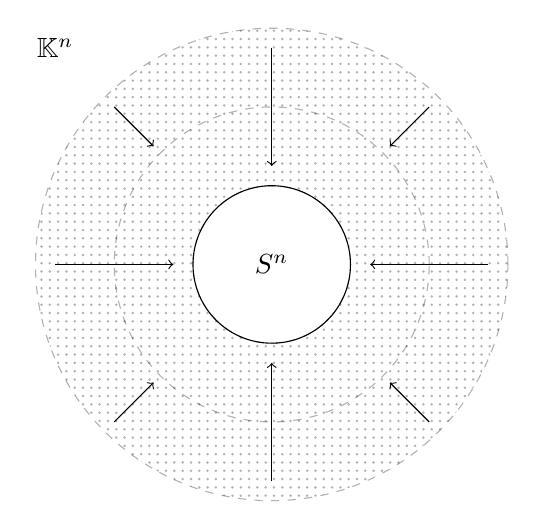
\begin{tikzpicture}
	\path[spath/save=Sn] (0,0) circle (1);
	\draw [pattern=dots, opacity=.3, dashed,
			% This line "isolates" Sn by reversing the path direction
		spath/insert reverse=Sn]
		(0,0) circle (3);
	\draw[opacity=.3, dashed] (0,0) circle (2);
	\draw (-2.75,2.75) node {$\mathbb{K}^n$};

		%long arrows
	\draw[->] (2.75,0) -- (1.25,0);
	\draw[->] (-2.75,0) -- (-1.25,0);
	\draw[->] (0,2.75) -- (0,1.25);
	\draw[->] (0,-2.75) -- (0,-1.25);

		%short arrows
	\draw[->] (2,2) -- (1.5,1.5);
	\draw[->] (-2,2) -- (-1.5,1.5);
	\draw[->] (2,-2) -- (1.5,-1.5);
	\draw[->] (-2,-2) -- (-1.5,-1.5);

	\draw (0,0) node {$S^n$} circle (1cm);
\end{tikzpicture}
\end{document}
